\documentclass[a4paper, final]{article}
\usepackage{cmap}
%\usepackage{literat} % Нормальные шрифты
\usepackage[14pt]{extsizes} % для того чтобы задать нестандартный 14-ый размер шрифта
\usepackage[T2A]{fontenc}
\usepackage[UTF8]{inputenc}
\usepackage[russian]{babel}
\usepackage{listings} %листинги
\usepackage{amsmath}
\usepackage{amssymb} % Для красивого значка пустого множества
\usepackage[left=25mm, top=20mm, right=20mm, bottom=20mm, footskip=10mm]{geometry}
\usepackage{ragged2e} %для растягивания по ширине
\usepackage{setspace} %для межстрочного интервала
\usepackage{indentfirst} % для абзацного отступа
\usepackage{moreverb} %для печати в листинге исходного кода программ
\renewcommand\verbatimtabsize{4\relax}
\renewcommand\listingoffset{0.2em} %отступ от номеров строк в листинге
\renewcommand{\arraystretch}{1.4} % изменяю высоту строки в таблице
\usepackage[font=small, singlelinecheck=false, justification=centering, format=plain, labelsep=period]{caption} %для настройки заголовка таблицы
\usepackage{listingsutf8}
\usepackage{xcolor} % цвета
\usepackage{hyperref}% для гиперссылок
\usepackage{enumitem} %для перечислений
\usepackage{titlesec}
\usepackage{graphicx}
\graphicspath{ {./Рисунки/} }
%\usepackage{float}
\usepackage{booktabs}
\usepackage{floatrow}
\usepackage{scalerel} % Stretching images
\usepackage[final]{pdfpages}

\definecolor{apricot}{HTML}{FFF0DA}
\definecolor{mygreen}{rgb}{0,0.6,0}
\definecolor{string}{HTML}{B40000} % цвет строк в коде
\definecolor{comment}{HTML}{008000} % цвет комментариев в коде
\definecolor{keyword}{HTML}{1A00FF} % цвет ключевых слов в коде
\definecolor{morecomment}{HTML}{8000FF} % цвет include и других элементов в коде
\definecolor{captiontext}{HTML}{FFFFFF} % цвет текста заголовка в коде
\definecolor{captionbk}{HTML}{999999} % цвет фона заголовка в коде
\definecolor{bk}{HTML}{FFFFFF} % цвет фона в коде
\definecolor{frame}{HTML}{999999} % цвет рамки в коде
\definecolor{brackets}{HTML}{B40000} % цвет скобок в коде





\AtBeginDocument{\renewcommand{\contentsname}{Содержание}}
\AtBeginDocument{\renewcommand{\refname}{Список источников}}

\floatsetup[table]{style=plain,capposition=bottom}
\setlist[enumerate,itemize]{leftmargin=1.2cm} %отступ в перечислениях

\hypersetup{colorlinks,
  allcolors=[RGB]{010 090 200}} %красивые гиперссылки (не красные)

% подгружаемые языки — подробнее в документации listings (это всё для листингов)
\lstloadlanguages{ [LaTeX] TeX}
% включаем кириллицу и добавляем кое−какие опции
\lstset{language =[LaTeX] TeX, % выбираем язык по умолчанию
extendedchars=true , % включаем не латиницу
escapechar = | , % |«выпадаем» в LATEX|
frame=tb , % рамка сверху и снизу
commentstyle=\itshape , % шрифт для комментариев
stringstyle =\bfseries} % шрифт для строк

\textheight=24cm % высота текста
\textwidth=16cm % ширина текста
\oddsidemargin=0pt % отступ от левого края
\topmargin=-1.5cm % отступ от верхнего края
\parindent=24pt % абзацный отступ
\parskip=0pt % интервал между абзацами
\tolerance=2000 % терпимость к "жидким" строкам
\flushbottom % выравнивание высоты страниц

\begin{document} % начало документа
\lstset{
  language=SQL, % Язык кода по умолчанию
  morekeywords={*,...}, % если хотите добавить ключевые слова, то добавляйте
  % Цвета
  keywordstyle=\color{keyword}\ttfamily\bfseries,
  %stringstyle=\color{string}\ttfamily,
  stringstyle=\ttfamily\color{red!50!brown},
  commentstyle=\color{comment}\ttfamily,
  morecomment=[l][\color{morecomment}]{\#},
  % Настройки отображения
  breaklines=true, % Перенос длинных строк
  basicstyle=\ttfamily\footnotesize, % Шрифт для отображения кода
  backgroundcolor=\color{bk}, % Цвет фона кода
  frame=single,xleftmargin=\fboxsep,xrightmargin=-\fboxsep, % Рамка, подогнанная к заголовку
  rulecolor=\color{frame}, % Цвет рамки
  tabsize=3, % Размер табуляции в пробелах
  % Настройка отображения номеров строк. Если не нужно, то удалите весь блок
  numbers=left, % Слева отображаются номера строк
  stepnumber=1, % Каждую строку нумеровать
  numbersep=5pt, % Отступ от кода
  numberstyle=\small\color{black}, % Стиль написания номеров строк
  % Для отображения русского языка
  extendedchars=true,
  literate={Ö}{ {\"O} }1
  {~}{ {\textasciitilde} }1
  {а}{ {\selectfont\char224} }1
  {б}{ {\selectfont\char225} }1
  {в}{ {\selectfont\char226} }1
  {г}{ {\selectfont\char227} }1
  {д}{ {\selectfont\char228} }1
  {е}{ {\selectfont\char229} }1
  {ё}{ {\"e} }1
  {ж}{ {\selectfont\char230} }1
  {з}{ {\selectfont\char231} }1
  {и}{ {\selectfont\char232} }1
  {й}{ {\selectfont\char233} }1
  {к}{ {\selectfont\char234} }1
  {л}{ {\selectfont\char235} }1
  {м}{ {\selectfont\char236} }1
  {н}{ {\selectfont\char237} }1
  {о}{ {\selectfont\char238} }1
  {п}{ {\selectfont\char239} }1
  {р}{ {\selectfont\char240} }1
  {с}{ {\selectfont\char241} }1
  {т}{ {\selectfont\char242} }1
  {у}{ {\selectfont\char243} }1
  {ф}{ {\selectfont\char244} }1
  {х}{ {\selectfont\char245} }1
  {ц}{ {\selectfont\char246} }1
  {ч}{ {\selectfont\char247} }1
  {ш}{ {\selectfont\char248} }1
  {щ}{ {\selectfont\char249} }1
  {ъ}{ {\selectfont\char250} }1
  {ы}{ {\selectfont\char251} }1
  {ь}{ {\selectfont\char252} }1
  {э}{ {\selectfont\char253} }1
  {ю}{ {\selectfont\char254} }1
  {я}{ {\selectfont\char255} }1
  {А}{ {\selectfont\char192} }1
  {Б}{ {\selectfont\char193} }1
  {В}{ {\selectfont\char194} }1
  {Г}{ {\selectfont\char195} }1
  {Д}{ {\selectfont\char196} }1
  {Е}{ {\selectfont\char197} }1
  {Ё}{ {\"E} }1
  {Ж}{ {\selectfont\char198} }1
  {З}{ {\selectfont\char199} }1
  {И}{ {\selectfont\char200} }1
  {Й}{ {\selectfont\char201} }1
  {К}{ {\selectfont\char202} }1
  {Л}{ {\selectfont\char203} }1
  {М}{ {\selectfont\char204} }1
  {Н}{ {\selectfont\char205} }1
  {О}{ {\selectfont\char206} }1
  {П}{ {\selectfont\char207} }1
  {Р}{ {\selectfont\char208} }1
  {С}{ {\selectfont\char209} }1
  {Т}{ {\selectfont\char210} }1
  {У}{ {\selectfont\char211} }1
  {Ф}{ {\selectfont\char212} }1
  {Х}{ {\selectfont\char213} }1
  {Ц}{ {\selectfont\char214} }1
  {Ч}{ {\selectfont\char215} }1
  {Ш}{ {\selectfont\char216} }1
  {Щ}{ {\selectfont\char217} }1
  {Ъ}{ {\selectfont\char218} }1
  {Ы}{ {\selectfont\char219} }1
  {Ь}{ {\selectfont\char220} }1
  {Э}{ {\selectfont\char221} }1
  {Ю}{ {\selectfont\char222} }1
  {Я}{ {\selectfont\char223} }1
  {\{}{ { {\color{brackets}\{} } }1 % Цвет скобок {
  {\} }{ { {\color{brackets}\} } } }1 % Цвет скобок }
}

% НАЧАЛО ТИТУЛЬНОГО ЛИСТА
\begin{center}
\hfill \break
\hfill \break
\normalsize{МИНИСТЕРСТВО НАУКИ И ВЫСШЕГО ОБРАЗОВАНИЯ РОССИЙСКОЙ ФЕДЕРАЦИИ\\
 федеральное государственное автономное образовательное учреждение высшего образования «Санкт-Петербургский политехнический университет Петра Великого»\\[10pt]}
\normalsize{Институт компьютерных наук и кибербезопасности}\\[10pt] 
\normalsize{Высшая школа технологий искусственного интеллекта}\\[10pt] 
\normalsize{Направление: 02.03.01 Математика и компьютерные науки}\\

\hfill \break
\hfill \break
\hfill \break
\large{Проектирование WEB приложений}\\
\large{Отчёт по курсовой работе на тему:}\\
\large{\textbf{«Электронный дневник»\\}}

\hfill \break
\hfill \break
\end{center}
 
\small{ 
\begin{tabular}{lrrl}
\!\!\!Студент, & \hspace{2cm} & & \\
\!\!\!группы 5130201/20102 & \hspace{2cm} & \underline{\hspace{3cm}} & Гаар В.С. \\\\
\!\!\!Преподаватель, \hspace{2cm} & & \\
\!\!\!к.т.н., доц. & \hspace{2cm} & \underline{\hspace{3cm}} &  Попов С.Г. \\\\
&&\hspace{5cm}
\end{tabular}
\begin{flushright}
<<\underline{\hspace{1cm}}>>\underline{\hspace{2.5cm}} 2025 г.
\end{flushright}
}

\hfill \break
\hfill \break
\begin{center} \small{Санкт-Петербург, 2025} \end{center}
\thispagestyle{empty} % выключаем отображение номера для этой страницы

% КОНЕЦ ТИТУЛЬНОГО ЛИСТА
\newpage

\tableofcontents

\newpage

\cleardoublepage
\phantomsection

\addcontentsline{toc}{section}{Введение}
\section*{Введение}
В данном отчете представлено выполнение лабораторной работы по дисциплине <<Проектирование WEB приложений>>. В качестве предметной области был выбран процесс использования электронного дневнивка в школах.
В ходе работы требуется формализовать выбранную предметную область при помощи:
\begin{enumerate}
    \item текстового описания;
    \item ER-диаграмм;
    \item Use case-диаграмм и описаний.
\end{enumerate}

\newpage
\section{Описание предметной области}

Рассматриваемая предметная область -- использование электронного дневника в школах. Электронный дневник представляет собой цифровую систему, предназначенную для автоматизации процессов ведения школьной документации, взаимодействия между учениками, родителями и учителями, а также для организации учебного процесса. Основная цель системы -- облегчить доступ к информации об успеваемости, расписании, домашних заданиях и других аспектах школьной жизни. Кроме того, электронный дневник способствует повышению прозрачности образовательного процесса и упрощает администрирование учебной деятельности.

\subsection{Основные сущности предметной области}

\textbf{Ученик} -- человек, имеющий профиль, зарегистрированный в системе электронного дневнивка, и обучающийся в образовательном учреждении, имеющим один из следующих типов:
\begin{enumerate}
  \item дошкольная образовательная организация;
  \item общеобразовательная организация;
  \item профессиональная образовательная организация;
  \item образовательная организация высшего образования.
\end{enumerate}

% на основании:
% \begin{itemize}
%   \item Приказа о зачислении (форма ОШ-1)
%   \item Личного дела с медицинской картой
%   \item СНИЛС и свидетельства о рождении
% \end{itemize}
Каждый ученик привязан к одному классу и изучает несколько предметов. Он получает оценки за выполненные задания, а также фиксирует выполненные домашние задания. Ученики могут просматривать своё расписание, получать уведомления об изменениях и получать сообщения от учителей в системе, где каждое сообщение содержит текст и дату отправки. Профиль ученика содержит сведения об успеваемости и посещаемости, доступные для просмотра родителям через систему.

\textbf{Родитель} -- законный опекун ученика. Подтверждение родства осуществляется через:
\begin{itemize}
  \item Свидетельство о рождении (сканированная копия в системе)
  \item Нотариальную доверенность для опекунов
\end{itemize}

У одного родителя может быть несколько детей-учеников. Родители имеют возможность контролировать успеваемость ребёнка, анализируя полученные оценки, пропуски занятий и выполненные домашние задания. Взаимодействие с учителями осуществляется через систему сообщений, в которой родители могут получать уведомления о поведении ребёнка, его успехах или замечаниях со стороны преподавателя.

\textbf{Класс} -- группа учеников одной ступени обучения, занимающихся по единой образовательной программе (базовой/углублённой) с единым календарным учебным графиком. Номер класса формируется из ступени обучения (цифра 1--11) и дополнительного идентификатора (буква А--Я). Класс является основной единицей организации учебного процесса. Каждый класс имеет своё расписание занятий, сформированное администрацией школы. В рамках класса ведётся журнал успеваемости и посещаемости, в котором фиксируются все оценки и замечания.

\textbf{Предмет} -- учебный курс, который изучается учениками в образовательном учреждении. Каждый предмет преподаётся в рамках определённых уроков, во время которых учитель излагает материал, задаёт домашние задания и контролирует знания учеников. В системе электронного дневника каждому предмету соответствует список домашних заданий, контрольных работ и оценок.

\textbf{Учитель} -- педагогический работник с квалификацией:
\begin{itemize}
  \item Диплом о высшем образовании (сканы в личном деле)
  \item Свидетельство о повышении квалификации (раз в 3 года)
  \item Электронная подпись для выставления итоговых оценок
\end{itemize}

Учитель назначается для проведения уроков в рамках учебного расписания и может курировать один из классов как классный руководитель. Он отвечает за ведение журнала, выставление оценок, контроль посещаемости и внесение комментариев по успеваемости учеников. Кроме того, учителя могут взаимодействовать с родителями через систему сообщений, предоставляя рекомендации и замечания.

\textbf{Сообщение} -- текстовое уведомление, используемое для взаимодействия между родителями, учениками и учителями. Сообщения могут включать замечания о поведении, уведомления о предстоящих мероприятиях, просьбы и обратную связь. В системе может быть реализован функционал групповых уведомлений и рассылок. Каждое сообщение привязывается к конкретному уроку и может содержать рекомендации для учеников и родителей.

\textbf{Урок} -- учебное занятие, включающее определённый предмет и временной интервал. К уроку может быть прикреплено сообщение, учебные материалы и домашнее задание. Учитель фиксирует тему занятия, отмечает присутствующих учеников, выставляет оценки и добавляет комментарии. Уроки проводятся по установленному расписанию, а их результаты записываются в журнал.

\textbf{Расписание} -- последовательность уроков для определённого класса, составляемая на каждый учебный день. Расписание доступно для просмотра ученикам, родителям и учителям. Оно включает информацию о преподавателях, предмете и времени начала занятий. В системе предусмотрена возможность оперативного обновления расписания при отмене или переносе уроков.

\textbf{Оценка} -- формализованный результат обучения; балл, выставленный за выполнение учеником учебной работы: 
\begin{itemize}
  \item Шкала: 2-5 с возможностью дробных значений (4+)
  \item Типы: текущая, рубежная, итоговая
  \item Весовой коэффициент (напр., контрольная — 40\%)
\end{itemize}
Оценки выставляются учителями и отображаются в профилях учеников.

\textbf{Домашнее задание} -- задание, выдаваемое ученикам для самостоятельного выполнения. Ученики записывают домашние задания, а учителя могут оценивать их выполнение. Домашние задания могут содержать ссылки на дополнительные материалы и задания с автоматической проверкой. Каждое домашнее задание связано с конкретным предметом и конкретным уроком, а по его выполнению ученик получает оценку.

\textbf{Администрация школы} -- группа сотрудников, ответственных за управление учебным процессом и функционирование системы электронного дневника:
\begin{itemize}
  \item Директор -- ответственный оператор персональных данных
  \item Завуч -- утверждает учебные планы и расписание
  \item Системный администратор -- обеспечивает ИБ
\end{itemize}

Администрация обеспечивает корректную работу системы, контролирует соблюдение образовательных стандартов и организует взаимодействие между всеми участниками учебного процесса.

\subsection{Основные процессы}
\noindent \textbf{Процесс ведения успеваемости}
\begin{enumerate}
  \item Учитель проводит урок и оценивает знания учеников.
  \item Оценки фиксируются в электронном дневнике.
  \item Ученики и родители могут просматривать оценки и получать уведомления о новых отметках.
  \item Учитель может добавлять комментарии к оценкам.
  \item Родители имеют возможность оставлять запросы на разъяснение выставленных оценок.
\end{enumerate}

\noindent \textbf{Процесс ведения расписания}
\begin{enumerate}
  \item Администрация школы формирует расписание для каждого класса.
  \item Расписание загружается в систему электронного дневника.
  \item Учителя и ученики могут просматривать расписание и получать уведомления об изменениях.
  \item В случае изменений администрация оперативно вносит корректировки.
\end{enumerate}

\noindent \textbf{Процесс выполнения домашних заданий}
\begin{enumerate}
  \item Учитель задаёт домашнее задание в системе.
  \item Ученик выполняет задание и загружает его в электронный дневник.
  \item Учитель проверяет работу и выставляет оценку.
  \item Ученик и родители могут просмотреть оценку и комментарии к выполненной работе.
\end{enumerate}

\noindent \textbf{Процесс контроля посещаемости}
\begin{enumerate}
  \item Учитель фиксирует присутствие учеников на уроке.
  \item В случае пропуска указывается причина отсутствия.
  \item Родители получают уведомление о пропущенных занятиях.
  \item Администрация школы анализирует посещаемость учеников.
\end{enumerate}

\noindent \textbf{Формирование отчётности}
\begin{enumerate}
  \item Учителя и администрация школы формируют отчёты об успеваемости и посещаемости учеников.
  \item Родители могут скачивать отчёты о результатах своего ребёнка.
  \item Отчёты могут быть экспортированы в различные форматы (PDF, Excel) для анализа и хранения.
\end{enumerate}


\subsubsection{Вспомогательные процессы}
\noindent \textbf{Регистрация и управление профилями}
\begin{enumerate}
  \item Ученик, родитель или учитель регистрируется в системе электронного дневника.
  \item Администрация школы подтверждает регистрацию.
  \item Участник получает доступ к своим данным.
  \item В случае необходимости пользователи могут изменять свои данные и пароли.
\end{enumerate}

\noindent \textbf{Обратная связь и взаимодействие}
\begin{enumerate}
  \item Учителя, родители и ученики могут обмениваться сообщениями в системе.
  \item Сообщения могут включать текст, файлы и мультимедийные материалы.
  \item Учителя могут отправлять уведомления о важной информации.
  \item Родители могут оставлять запросы на разъяснение оценок и дисциплинарных мер.
\end{enumerate}


\noindent \textbf{Настройки и администрирование системы}
\begin{enumerate}
  \item Администраторы школы могут управлять правами доступа пользователей.
  \item Учителя могут добавлять методические материалы и учебные планы.
  \item Система может интегрироваться с другими образовательными платформами.
  \item Обновления и изменения в системе регулярно вносятся для улучшения функционала.
\end{enumerate}
  
Таким образом, электронный дневник играет важную роль в организации учебного процесса, облегчая взаимодействие между всеми участниками образовательного процесса и обеспечивая удобный доступ к важной информации.

\newpage
\section{ER-диаграмма}
\subsection{Абзац}
\textbf{Ученик} -- человек, имеющий профиль, зарегистрированный в системе электронного дневнивка, и обучающийся в образовательном учреждении, имеющим один из следующих типов:
\begin{enumerate}
  \item дошкольная образовательная организация;
  \item общеобразовательная организация;
  \item профессиональная образовательная организация;
  \item образовательная организация высшего образования.
\end{enumerate}
Также каждый ученик привязан к одному классу и изучает несколько предметов. Он получает оценки за выполненные задания и фиксирует выполненные домашние задания. Ученики могут просматривать своё расписание, получать уведомления об изменениях и получать сообщения от учителей в системе, где каждое сообщение содержит текст и дату отправки. Профиль ученика содержит сведения об успеваемости и посещаемости, доступные для просмотра родителям через систему.

ER-диаграмма представлена на \hyperlink{diag:er}{рисунке №1}.

\newpage
\hypertarget{diag:er}{}
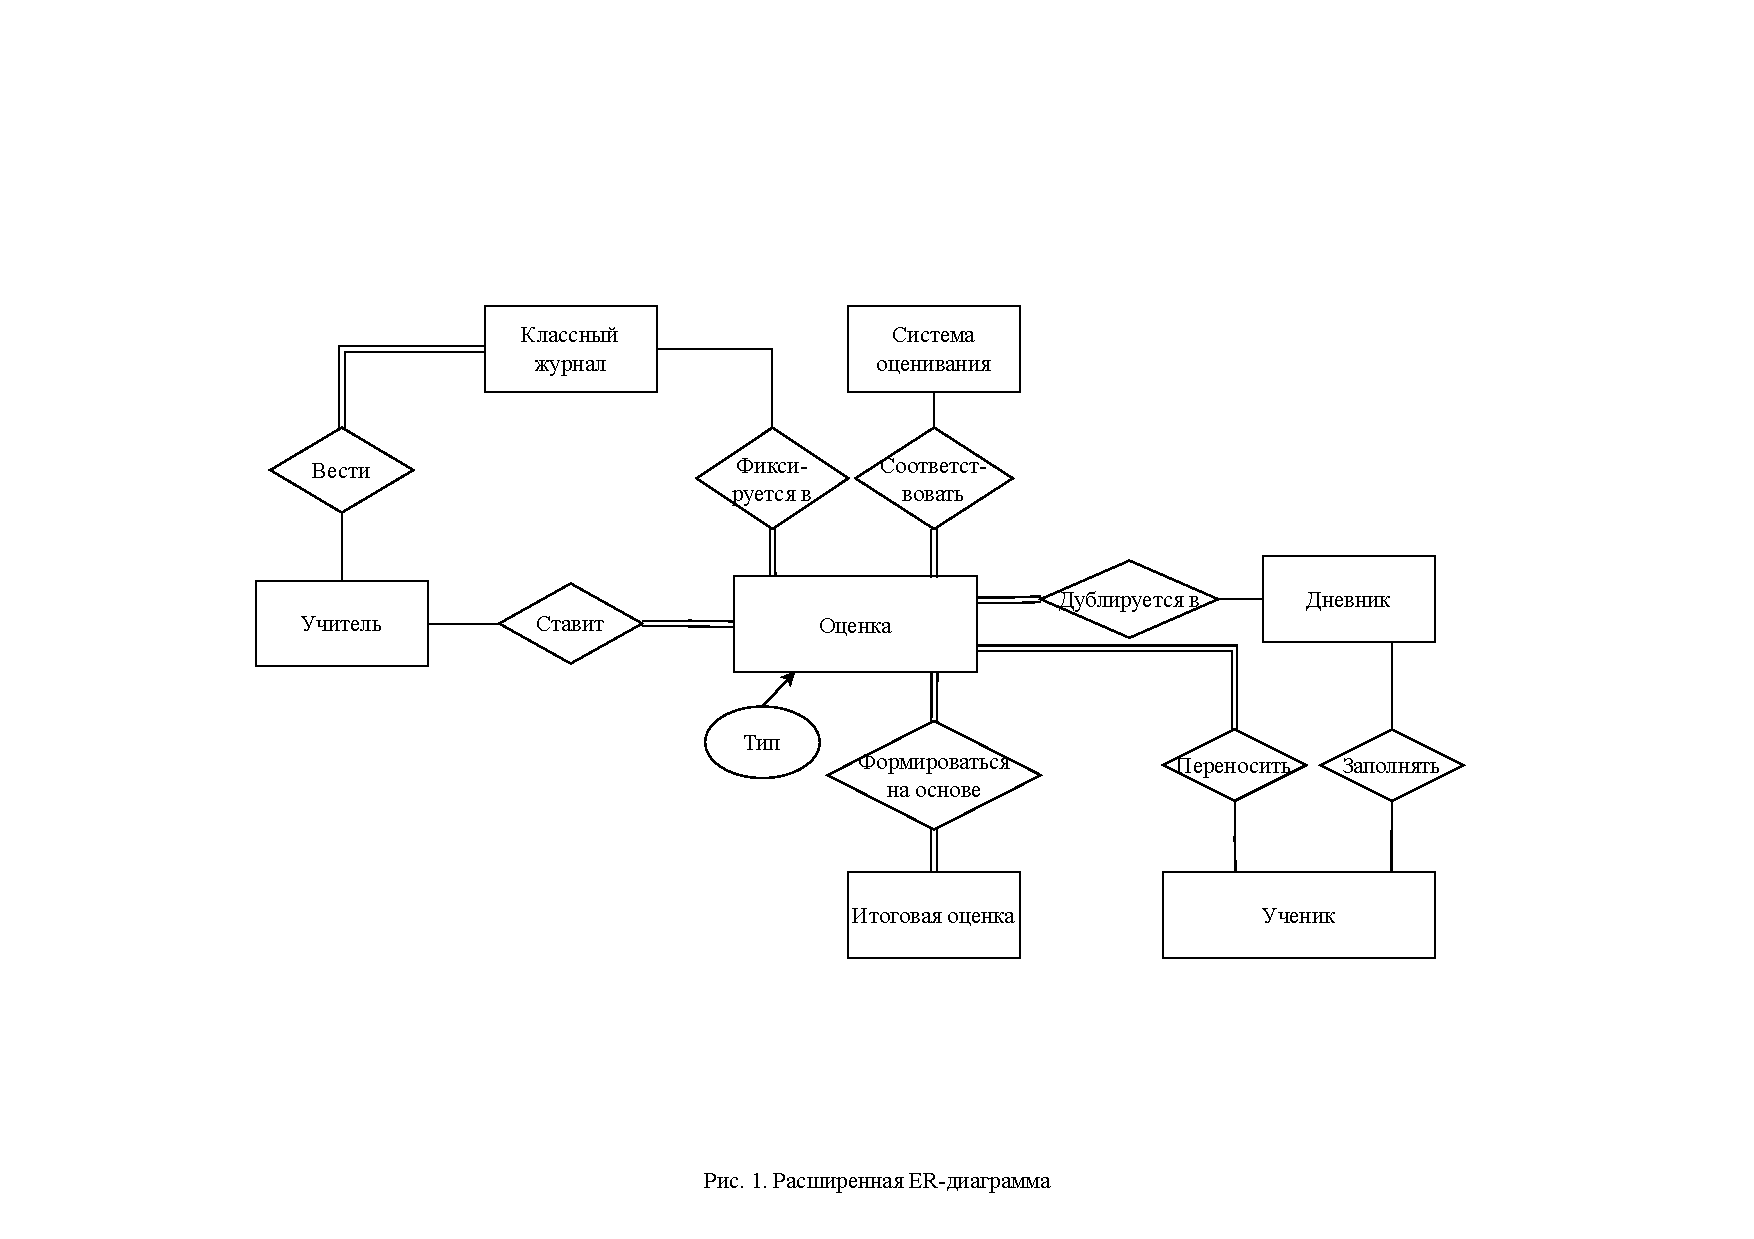
\includepdf[pages=1, fitpaper]{Рисунки/ER.pdf}
\addtocounter{figure}{1}
\newpage

\subsection{Чтение ER-диаграммы}
Каждый ученик имеет собственный профиль, зарегистрированный в системе электронного дневнивка, и обучается в образовательном учреждении со своим типом. Каждый ученик привязан к одному классу и изучает несколько предметов. Ученики получают оценки за выполненные задания и фиксируют выполненные домашние задания. Ученики могут просматривать расписание, получать уведомления и сообщения от учителей. Учителя могут отправлять сообщения ученикам. Сообщения содержат текст и дату отправки. Профиль ученика содержит сведения об успеваемости и посещаемости, а профиль ученика со всеми сведениями доступен для просмотра родителям через систему.



\newpage
\section*{Заключение}
\addcontentsline{toc}{section}{Заключение}
Полученные знания могут быть и будут использованы в работе над последующими проектами и заданиями.

\cleardoublepage
\phantomsection
\newpage
%Список источников
\begin{thebibliography}{0}
	% \bibitem{bib:mysqldoc}
	% MySQL Documentation [Электронный ресурс] URL: https://dev.mysql.com/doc/ (дата обращения 30.04.2024).
\end{thebibliography}
\addcontentsline{toc}{section}{Список источников}
\end{document}